\chapter{Evaluation}
\label{cha:evaluation}

Per la valutazione del bot ho deciso di eseguire alcuni \textit{usability testing}. Questa metodologia consiste in sessioni di osservazione diretta, non intrusiva, dell’interazione tra un utente e un servizio digitale. Durante il test vengono assegnati all’utente uno o più task da svolgere, il compito dell’osservatore è quello di analizzare il comportamento nel portarli a termine. Unito a questo tipo di test, utilizzerò il think aloud. Questa metodologia, come suggerisce il nome, richiede all'utente di esprimere a parole e ad alta voce quali sono i suoi pensieri, le sue azioni, le sue intenzioni e le difficoltà incontrate durante l'interazione con l’interfaccia.


Due dei quattro utenti sono stati selezionati a partire dalla popolazione che utilizza il bot, mentre gli altri non avevano mai interagito con esso prima del test. 

\noindent Le operazioni che ho chiesto di svolgere sono:
\begin{itemize}
    \item trovare il bot e avviarlo;
    \item cercare la fermata dell'autobus urbano "Maccani rotatoria";
    \item salvare la fermata nei preferiti;
    \item visualizzare la corsa precedente e successiva;
    \item visualizzare la lista delle fermate; 
    \item ritornare al menu principale; 
    \item visualizzare la propria lista delle fermate preferite;
    \item visualizzare la situazione delle stazioni di ricarica delle bici;
    \item visualizzare il tabellone delle partenze della fermata Mezzocorona della ferrovia del Brennero.
\end{itemize}

\begin{wrapfigure}{r}{0.38\textwidth}
\centering
\frame{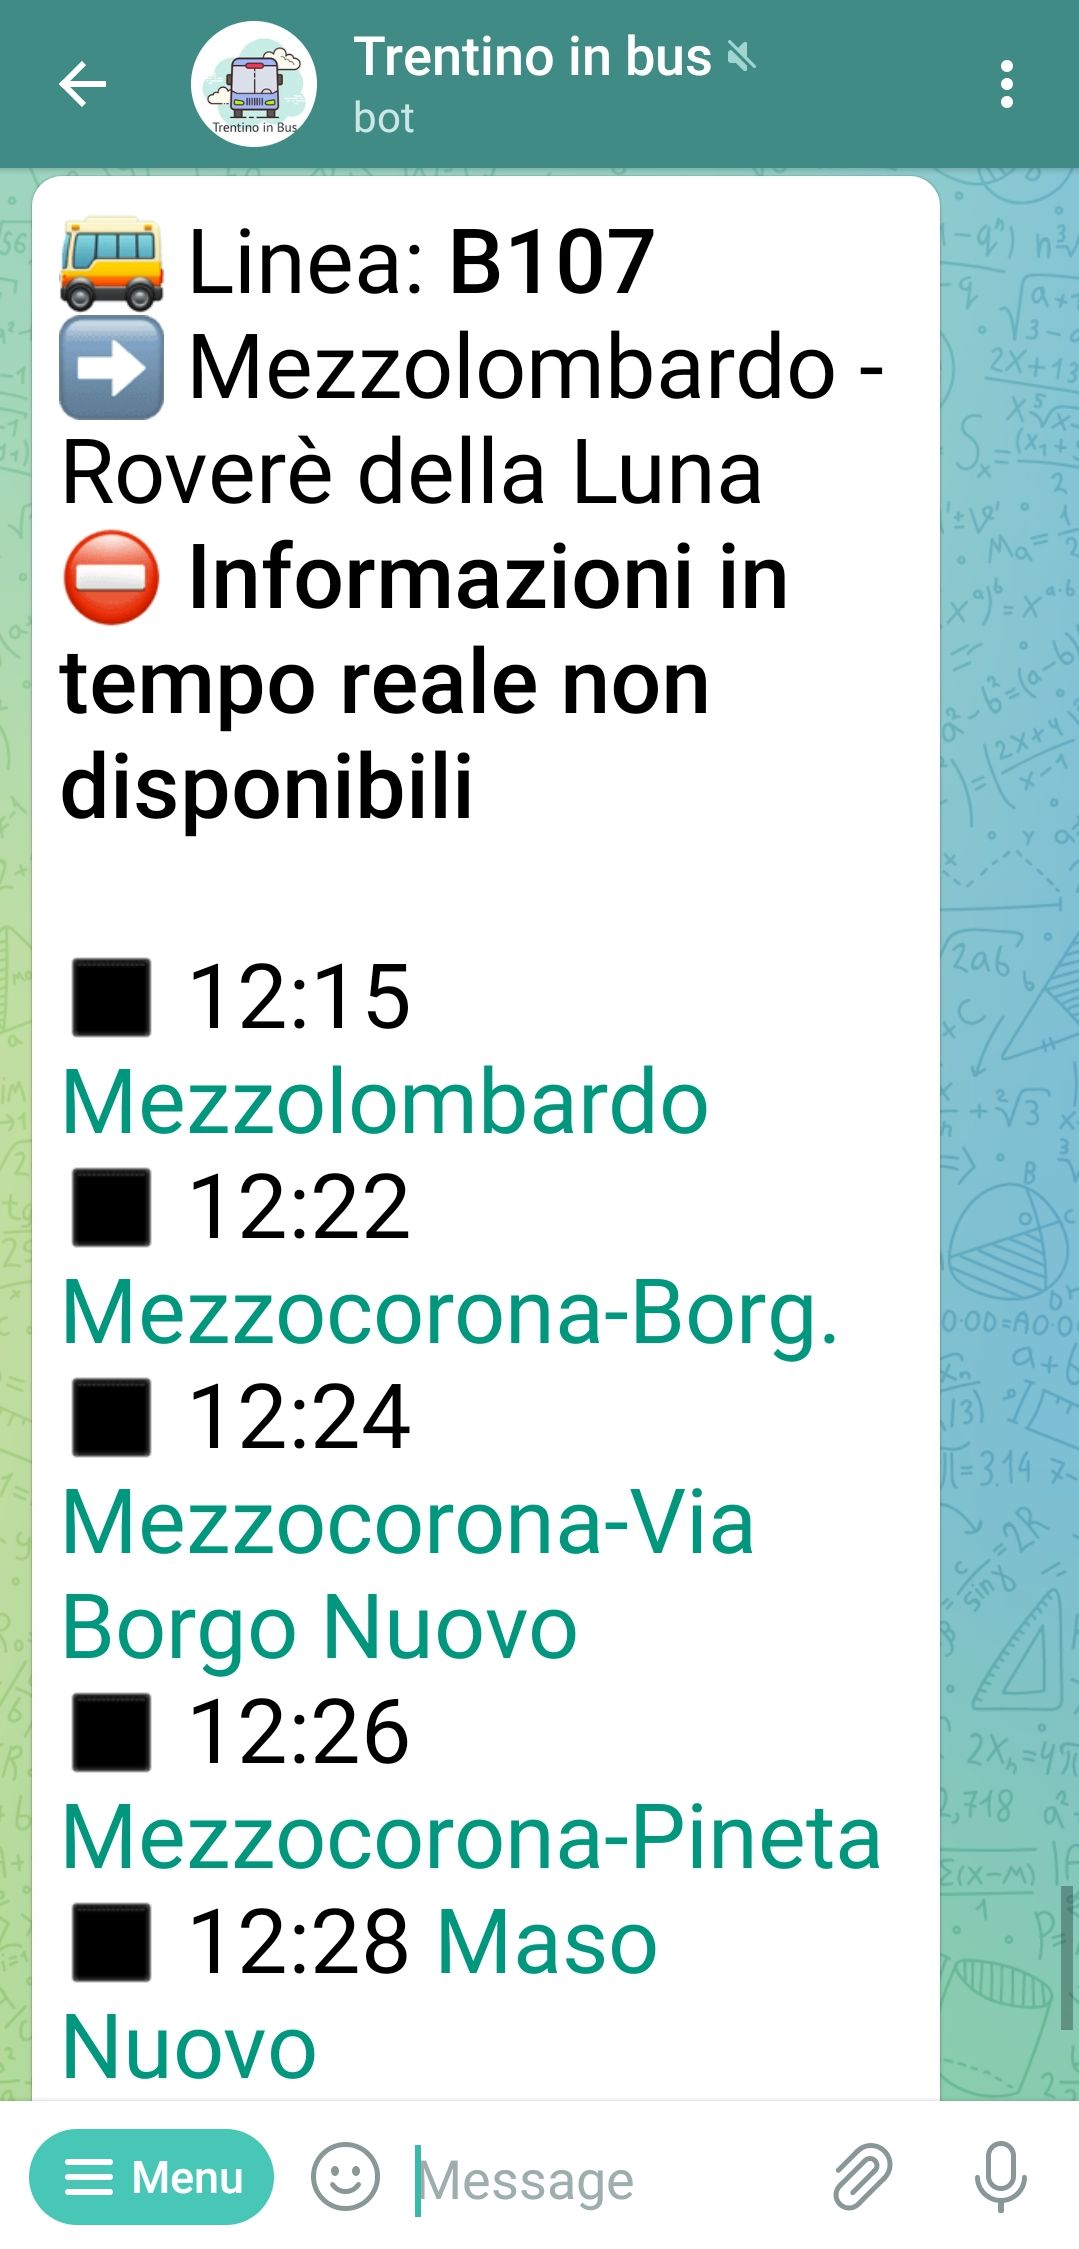
\includegraphics[scale=0.09]{bot-large-font.jpg}}
\caption{Problema formattazione}
\label{fig:bot-large-font}
\end{wrapfigure}


Dagli usability testing è emerso che, data la presenza dei tasti, che permettono una divisione in sezioni delle diverse abilità, delle emoji e i messaggi guida che appaiono durante l'utilizzo; sia l'utente con esperienza che quello inesperto riescono a muoversi con intuitività tra le varie sezioni del bot, eseguendo facilmente i task richiesti. 
Una difficoltà che ho notato è che la dimensione dei caratteri del singolo dispositivo influiscono sulla chiarezza dell'interfaccia, questo perché, come è possibile notare in figura \ref{fig:bot-large-font}, una dimensione molto grande del testo provoca dei problemi alla formattazione delle tabelle orario. Questo è stato sottolineato anche dalla difficoltà  presentata da un utente durante il task di visualizzazione degli orari della fermata urbana. Sfortunatamente, questa è una limitazione della piattaforma Telegram ed è impossibile risolverla se non avvertendo l'utente di questa situazione. 

Successivamente, una volta eseguito il test, ho chiesto agli utenti se avessero dei miglioramenti che avrebbero voluto vedere nel bot. Uno degli utenti, in particolare, ha risposto 
\textit{"Si potrebbe migliorare il monitoraggio delle bici, differenziando tra bici elettriche e non."}. Sempre riguardo questa funzionalità, un altro utente suggerisce di inserire la possibilità di ricercare la stazione di ricarica più vicina alla propria posizione. 
Altre idee che sono state avanzate riguardano l'inserimento della possibilità di acquisto di biglietti per il servizio di trasporti provinciale, e la ricerca dei percorsi data una partenza e una destinazione.


